\section{Class diagrams}
\twopagepicture{b}{l}{figures/CommonLayer}{Class diagram common layer}
\subsubsection{Common layer}
The \texttt{CommonLayer} is shown in figure 2. The design of the classes are in mind that it can be shared in between layers and it can be serialized (written to file). Hence the class diagram follow the constraints that it can't use any interfaces or that there is a circular reference (it has to look like a tree). Notice that the 
\texttt{PedestrianEntity} and the \texttt{CarEntity} are in an \texttt{ObservableCollection} and have observable attributes. When the simulation is running the view will be be notified when attributes are changed.

\subsection{View layer}
In figure \ref{fig:pres} the class diagram of the view layer is shown. Inside of the view we do not use the usual \texttt{Graphics} used in Forms application to draw on the screen but instead a \texttt{Canvas} to draw on the screen. A lot of the drawing is already handled and we have especially bind the right values.

\subsection{Business Layer}
In figure \ref{fig:bus} the class diagram of the business layer is shown. We choose to make operations for adding and deleting components instead of using an observable collection since by using operations is more simple to maintain business rules. 

\subsection{Data Layer}
In figure \ref{fig:data} the class diagram of the data layer is shown. The data layer does not show concrete implementation since the classes don't require to have a state.

\newpage
\begin{figure}[!ht]
	\centering
	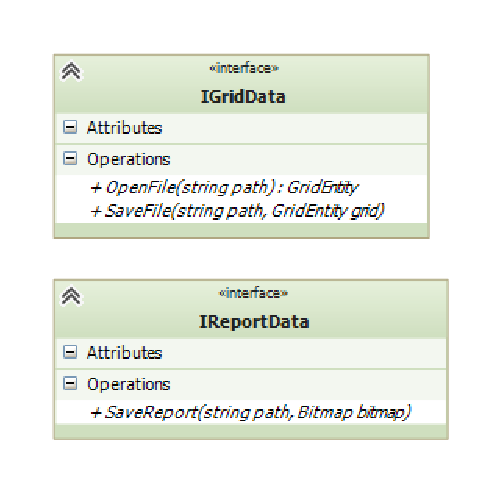
\includegraphics{figures/DataLayer}
	\caption{Class diagram data access layer}
	\label{fig:data}
\end{figure}



\begin{landscape}
	\begin{figure}[!ht]
		\centering
		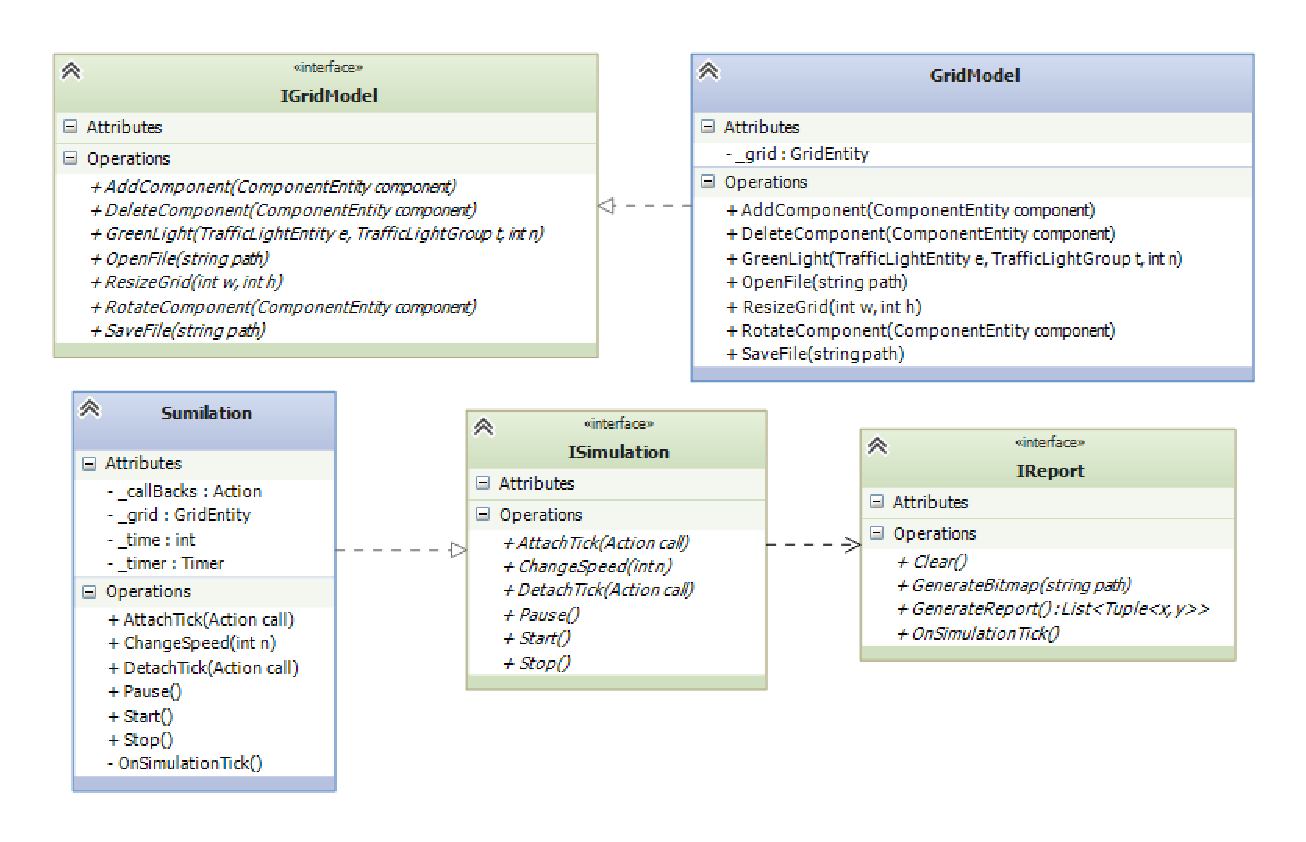
\includegraphics[height=\textheight]{figures/BusinessLayer}
		\caption{Class diagram business layer}
		\label{fig:bus}
	\end{figure}
\end{landscape}

\begin{landscape}
	\begin{figure}[!ht]
		\centering
		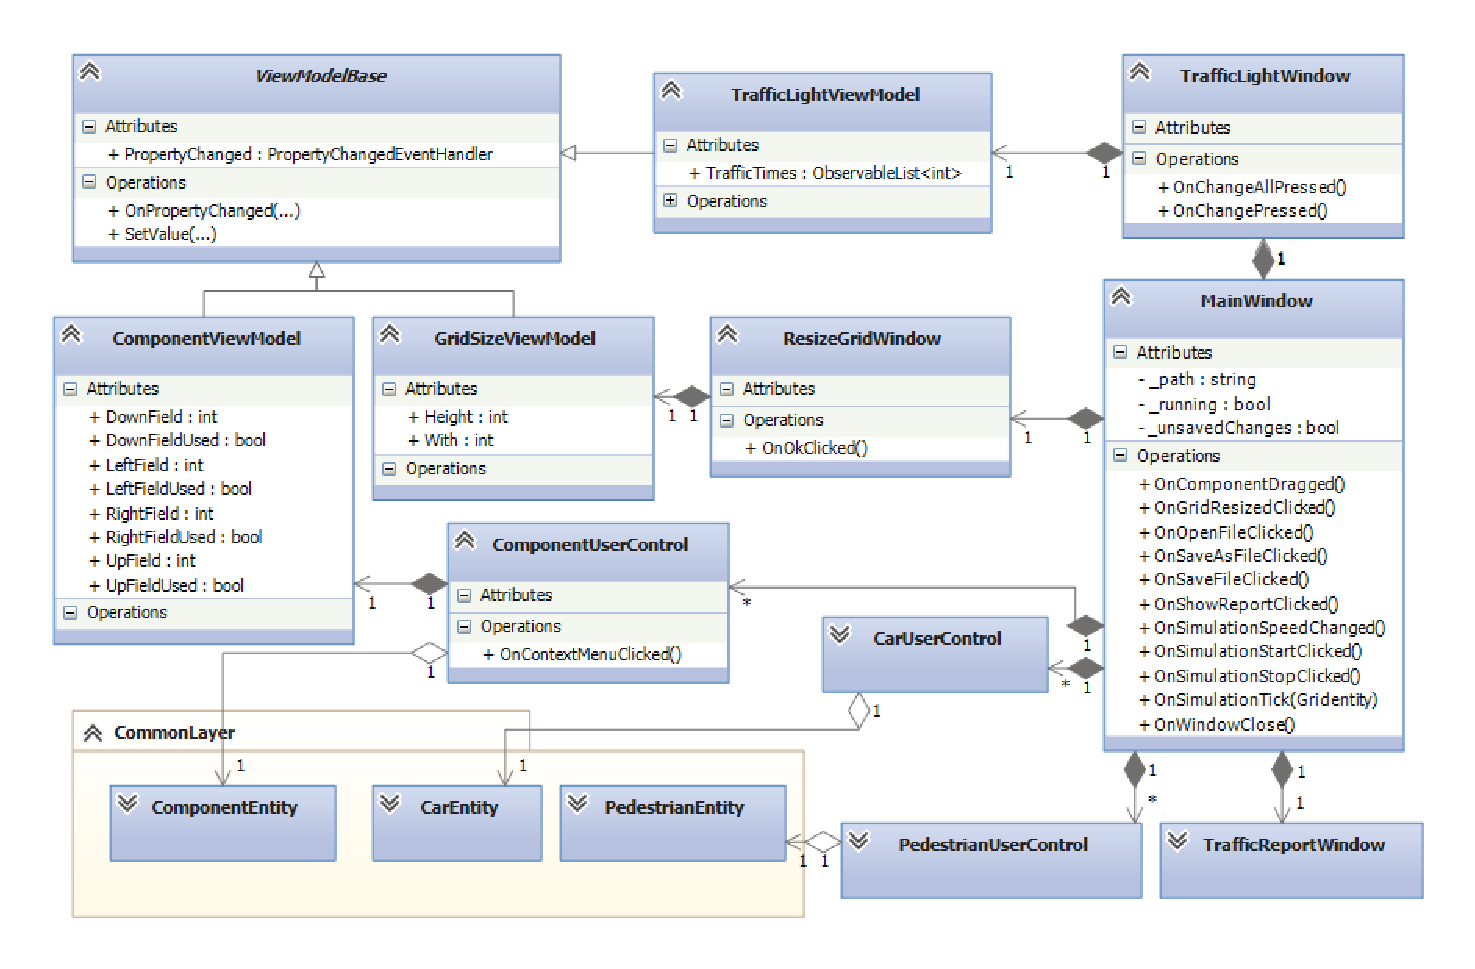
\includegraphics[height=\textheight]{figures/PresentationLayer}
		\caption{Class diagram view layer}
		\label{fig:pres}
	\end{figure}
\end{landscape}




